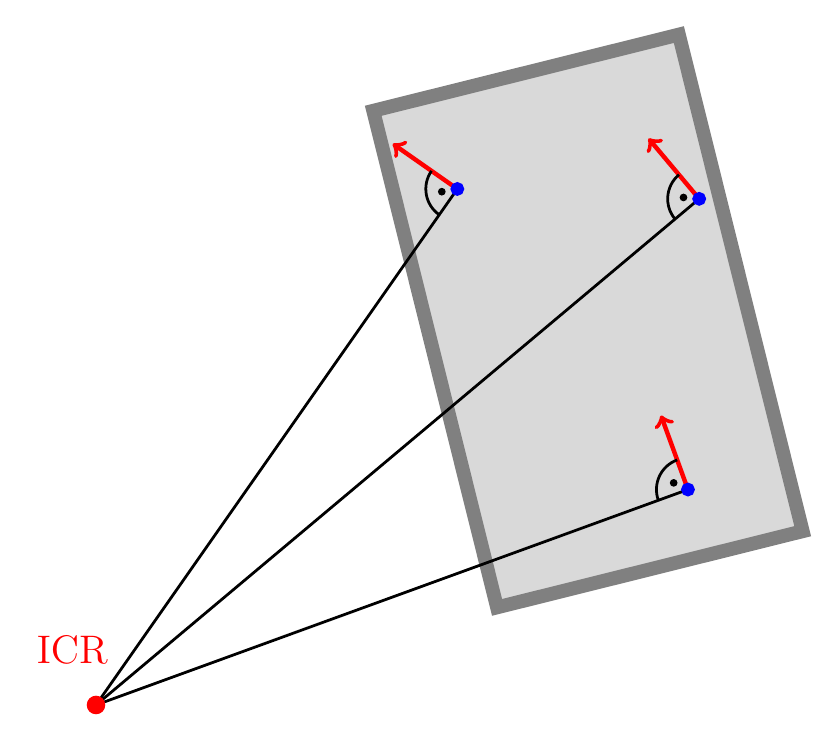
\begin{tikzpicture}[line width=1.0]
\usetikzlibrary{shapes.misc,shadows}
\usetikzlibrary{calc}
\usetikzlibrary{positioning,backgrounds}

\pgfmathsetmacro{\ArrowLength}{1}
\pgfmathsetmacro{\vheight}{4.5}
\pgfmathsetmacro{\vwidth}{2}
\pgfmathsetmacro{\deltavar}{15}
\pgfmathsetmacro{\xdist}{6}

\pgfmathsetmacro{\myrot}{14}
\pgfmathsetmacro{\myshift}{1}
%\pgfmathsetmacro{\myrot}{0}
%\pgfmathsetmacro{\myshift}{0}
\begin{scope}[shift={(0,\myshift)},rotate=\myrot]
	
% RECTANGLE			
\draw [line width = 5, gray, fill=gray!30!white] (-1+\xdist,-1) rectangle (\xdist+\vwidth+1,\vheight+1);

\end{scope}

%\draw[line width=2, color=blue]  (tire1.center) -- (tire2.center); 




\foreach \x/\y in {7.1/3.2, {\xdist+\vwidth}/0} {
  %\draw[] (0,0) -- (\x,\y);
  %/draw[->] (\x,\y) -- ({\atan({\y/\x})}, \sin(\x));
}


% radius R and angle P for right bottom (rb)
\pgfmathsetmacro{\Rrb}{  sqrt( (\xdist+\vwidth)^2 }
\pgfmathsetmacro{\Prb}{  0 }

% radius R and angle P for right top(rt)
\pgfmathsetmacro{\Rrt}{  sqrt( (\xdist+\vwidth)^2 +(\vheight)^2 }
\pgfmathsetmacro{\Prt}{  atan( \vheight / (\xdist+\vwidth) }


\foreach \r/\phi in {10/40, 8/20, 8/55} {

\pgfmathsetmacro{\x}{  \r*cos(\phi)   }
\pgfmathsetmacro{\y}{  \r*sin(\phi)   }

  \draw[] (0,0) -- (\x,\y);
  \draw[->, red, line width = 1.6] (\x,\y) -- ( {\x -sin(\phi)*\ArrowLength}, {\y + cos(\phi)*\ArrowLength});

  \draw[color=black] ({\x - sin(\phi)*0.4*\ArrowLength}, {\y + cos(\phi)*0.4*\ArrowLength}) arc ({90+\phi}:{180+\phi}:0.4*\ArrowLength);

  \draw[fill] ({\x - 0.2*\ArrowLength* sin(\phi+45)},{\y+0.2*\ArrowLength*cos(\phi+45)}) circle (0.03);
  \draw[fill, blue] (\x,\y) circle (0.07);
}


% top left
%\draw[ultra thick, green,->] (0, \vheight) -- ({0-sin(\deltavar)*\ArrowLength},{\vheight+\ArrowLength)});


 %angle delta left
%\draw[color=black] ({\ax+2},0) arc (0:\deltavar:2);
%\draw (\ax+1.3, 0.3) node[black] {$\delta$};
 
% circular arc
 %\draw[thick, ->] (0,0) arc (0:40:-\ax); 

% ICR
\node[red] at (-0.3,0.7){\Large ICR};
\draw[red, fill] (0,0) circle(0.1);



\end{tikzpicture}